% %%%%%%%%%%%%%%%%%%%%%%%%%%%%%%%%%%%%
% A LaTeX template for the technical essay of TTM4137 Wireless Security
% Stig F. Mjolsnes, 01.09.2012
%%%%%%%%%%%%%%%%%%%%%%%%%%%%%%%%%%%%%
\documentclass[a4paper,11pt]{article}

\usepackage[plain]{fullpage}
\usepackage{graphicx}  %This enables the inclusion of pdf graphic files in figures
\usepackage[hidelinks]{hyperref} % Make links in your document click-able NB: must be loaded before the caption-package
\usepackage{caption}
\usepackage{subcaption}
\usepackage{wrapfig} 


\title{BankID and two-factor authentication.}
\author{Anders Kofoed \\
	\texttt{anderkof@stud.ntnu.no}\\
	TTM4137 Wireless Security Technical Essay}
\date{\today}

\begin{document}
\maketitle

\section{Introduction}
Security in the world of e-commerce is an important issue. The Norwegian banking community has developed an solution called BankID, utilising two-factor authentication and a PKI model. The idea behind BankID is thought out well, the banking community aims to make BankID a national identification system, providing authentication as well as digital signatures. But is the implementation of the system that well enough thought trough, and are there weaknesses to be exploited? This essay will explain how the system is built, and identify some of the challenges faced by the BankID project. I will try to focus on the two-factor authentication part of the system to a larger extent. 


\section{Problem Discussion}
\begin{wrapfigure}[18]{r}{0.45\textwidth}
  \centering
  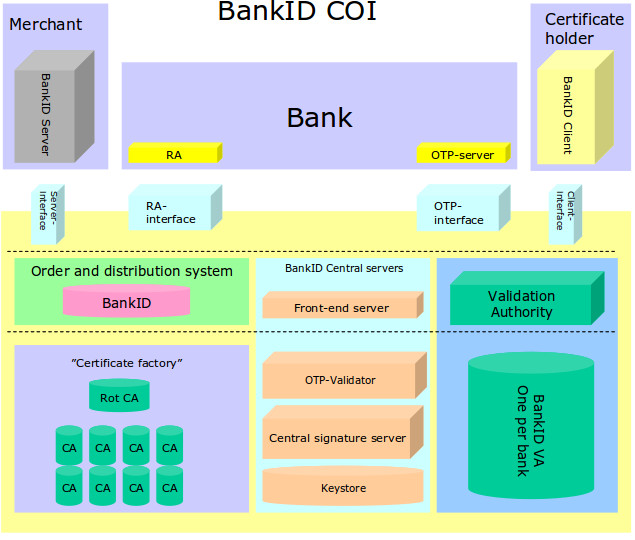
\includegraphics[scale=0.35]{architecture} %Note: no use of .jpg file ending
  \vspace{-0.2cm}
  \caption{BankID architecture.}
  \label{fig:arch}
\end{wrapfigure}
\subsection{Architecture of the BankID system.}
\paragraph{PKI, public key infrastructure} is often the preferred model for efficient and secure online services. Often accompanied by the use of several factors of authentication. The background for this approach is the guidance entitled \emph{Authentication in an Internet Banking Environment} \cite{auth-banking}. PKI is a widely used technique used to provide public encryption and verification(digital signatures). The normal way of implementing a PKI, is by supplying each entity with their own private key, whom only they have control of. And then distribute the corresponding public key used to verify signatures and encrypt data. The variation deployed by BankID, is that the private keys is stored locally and in control of the banks. I will come back to how this simplification contradicts basic requirements of digital signatures in PKI. The BankID system simplifies this structure by storing the signing keys locally, and then make, or verify, signatures on request from the user. The total architecture is shown in {figure~\ref*{fig:arch}}. The architecture consists of 4 main components\cite{whitepaper}:
\begin{itemize}
  \item Certificate holder: A user possessing a BankID, requesting something to be signed or verified.
  \item Merchant: Some kind of online service using BankID identification or signing.
  \item Certificate issuer: A bank issuing BankID with responsibility for maintenance (issuing, revoking and renewal) of the BankIDs.
  \item Certificate validation: Service provided normally by the providers of BankID. Used to verify signatures. 
\end{itemize}
 The main idea of this architecture is to enable two parties without a trusted relationship to establish a secure communication channel. We see that the establishment of the channel is done through a third party which both communicating parties trust. In classical PKIs this third party is a certificate authority (CA), which issues a certificate associating a public key to the recipient. In BankID, the public-private key pair is generated by the central infrastructure on request from the banks, typically when a new user is registered with BankID by the bank. The private key is stored in a central database as mentioned, while the public key is stored at the CA related to the customer's bank. When a user wants to use the BankID client, a Java applet in the browser is used. The user is advised to check the certificate of this page, to assure the user of the authenticity of the web page, and avoid phishing attacks (will be discussed later). The user then authenticates with the server, and gives the central infrastructure access to the stored keys. Next, the infrastructure executes the actions requested (signing or encrypting something). The BankID server, being online stores or similar merchants can then verify the signed challenge received from the client and vice versa. \cite{bankid}
 

\paragraph{Two-factor authentication} is used to obtain authentication between the bankID client and server. First the user enters his social security number which is used to generate a list of the users associated BankIDs (it is possible to have several). Then the client prompts the user for a one time password, generated by a password-generating token issued by the bank. 


\subsection{Security Capabilities}

\subsection{Vulnerabilities and Limitations.}




\section{Conclusion}
The submitted technical essays will be graded and contribute 20\% to the final grade of the course. The two best essays will be honoured with publication at It's learning, edited if necessary and become part of this year's  syllabus.



\begin{thebibliography}{N}\label{sec:references}

\bibitem{auth-banking} Federal Financial Institutions Examination Council  \textit{Authentication in an Internet Banking Environment} 13-Sep-2011 \url{http://www.digitallibrary.kcci.com.pk/handle/32417747/701}

\bibitem{whitepaper} Bankenes BetalingsSentral AS \textit{BankID COI White Paper} 05.09.2005 \url{http://www.eurim.org.uk/activities/pi/BankIDWhitePaper.pdf}

\bibitem{bankid}  Professor K. J. Hole, Department of Informatics, University of
Bergen \textit{Next Generation Internet Banking in Norway} \url{https://bora.uib.no/bitstream/handle/1956/2636/Dr.Avh._Thomas_%20Tjostheim.pdf?sequence=1#page=141}

\bibitem{attack1}NoWires Research Group, Department of Informatics UiB \textit{A Proof of Concept Attack against Norwegian Internet Banking Systems} Short paper version, Feb. 21st, 2008.

\bibitem{weakness1}Kristian Gjøsteen Department of Mathematicla Science and Technology, NTNU \textit{Weaknesses in BankID, PKI-Substitute Deplayed by Norwegian Banks.} 2008



\end{thebibliography}

\end{document} 
